\documentclass[10pt,letterpaper]{article}
\usepackage[utf8]{inputenc}
\usepackage[english]{babel}
\usepackage{amsmath}
\usepackage{amsfonts}
\usepackage{amssymb}
\usepackage{graphicx}
\graphicspath{{../Figures/}}
\usepackage{hyperref}
\usepackage{apacite}
\usepackage{booktabs}
\usepackage{subcaption}
\usepackage[left=2cm,right=2cm,top=2cm,bottom=2cm]{geometry}
\setlength{\parskip}{\baselineskip}%
\setlength{\parindent}{0pt}%

\usepackage[compact]{titlesec}
\titlespacing{\section}{0pt}{*0}{*0}
%\titlespacing{\subsection}{0pt}{*0}{*0}
%\titlespacing{\subsubsection}{0pt}{*0}{*0}

\author{Silas Mann \and Jonas Peeters}
\title{DS-GA 1017 Project: Fairness in Sepsis Detection}
\date{\today}
\begin{document}
\maketitle
\vspace*{-1cm}

% \pagenumbering{gobble}

% DRAFT BACKGROUND AND INPUT AND OUTPUT SECTIONS

\section*{Background}

% 1. Background: general information about your chosen ADS
%	a. What is the purpose of this ADS? What are its stated goals?
%	b. If the ADS has multiple goals, explain any trade-offs that these goals may introduce.

\par Sepsis is a life-threatening dysfunctional immune response to infection in which the body attacks its own tissues and organs, often leading to organ failure and death \cite{Singer2016}. It is a critically important world-wide public health issue; with a mortality rate of about 16\%, the estimated number of world-wide cases is as high as 31.5 million \cite{Fleischmann2016}, and in the United States alone over 1.7 million develop sepsis annually\footnote{\href{https://www.cdc.gov/sepsis/clinicaltools/index.html?CDC_AA_refVal=https\%3A\%2F\%2Fwww.cdc.gov\%2Fsepsis\%2Fdatareports\%2Findex.html}{https://www.cdc.gov/sepsis/clinicaltools.html}}. Better outcomes and lower mortality rates have been connected to early treatment, including the administration of early antibiotics and fluids \cite{Rhee2018}. However, early identification of sepsis remains a challenge. Much work has been done in an effort to develop early identification strategies in the clinical setting \cite{Kim2019}, and in recent years, these efforts have turned toward the use of automated decision systems based on machine learning to predict sepsis \cite{Fleuren2020} and identify patients who may benefit from treatment programs such as early-goal directed therapy (EGDT) or SSC bundles \cite{Kim2019}. In an effort to advance these efforts, PhysioNet, a repository for freely-available medical research data, launched a 2019 challenge entitled “Early Prediction of Sepsis from Clinical Data” \cite{Reyna2019}.

\par The use of machine learning models to assess the state of patients' health and determine whether to initiate preemptive procedures is relatively new. In the case of sepsis, if the model is able to correctly predict risk, it has the opportunity to prevent life-threatening illness. If the model fails to predict risk, the consequences can be grave. If the model incorrectly predicts sepsis, vital resources may be allocated to a patient that would have better allocated to another patient. Additionally, frequent incorrect predictions can result in alert fatigue; doctors may choose to ignore the predictions if they tend to be incorrect.  Given the gravity of the consequences, it is paramount that such models do not further perpetuate differences in medical treatment between protected groups. For example, \citeauthor{Greenwood2018} found that female patients are less likely than their male counterparts to survive traumatic health episodes such as heart attacks. A model that informs doctors on the risk of sepsis could either reinforce existing biases in medical care or potentially lessen them by offering a more impartial assessment than may be provided by the largely male medical staff found in ICUs \cite{Chadwick2020}.

\par In 2019, \citeauthor{Sindwani2019} published an article in Towards Data Science titled “Early Detection of Sepsis Using Physiological Data". In the article, the author outlines the problem above. He shows the results of exploratory data analysis, feature selection/engineering, and model training and evaluation. The author also provides a link to a fully functioning GitHub \cite{Karan2019}. In our analysis for fairness, we chose the best model provided by the author. 

\par First, we determine if there are any currently existing biases on the basis of gender or age which may lead to less favorable outcomes for marginalized groups. Here we explore disparate impact and mean difference between the predictions for both the privileged and unprivileged groups. Next, we look at the pre-processing steps taken by the author, and identify any steps that introduce additional bias. We then explore the results of the model, and analyze whether the model will introduce or perpetuate any bias between groups, again using disparate impact and mean difference as our metrics. Most medical data are provided at the level of the individual patient, and several precautions are taken to ensure the privacy of the individuals included in the data set. Therefore we have also analyzed the possible pitfalls of the privacy measures implemented in this data set.

\section*{Input and output}

% 2. Input and output
%	a. Describe the data used by this ADS. How was this data collected or selected?
%	b. For each input feature, describe its datatype, give information on missing values and on the value distribution. Show pairwise correlations between features if appropriate. Run any other reasonable profiling of the input that you find interesting and appropriate.
%	c. What is the output of the system (e.g., is it a class label, a score, a probability, or some other type of output), and how do we interpret it?

\par The training data, which were provided in the PhysioNet website to anyone interested in participating, were sourced from 40,000 ICU patients from Beth Israel Deaconess Medical Center and Emory University Hospital. While the test data do not appear to have ever been released, the training data are still available for download in the PhysioNet archive \cite{Goldberger2000}. The deidentified data for each patient is contained within a single pipe-delimited file, and include demographics, vitals, and laboratory values, and defined binary sepsis onset based on relevant events (time of initial clinical suspicion, time of deterioration in organ failure assessment, and time of sepsis onset).

\par Time of initial clinical suspicion of infection was defined as either the time IV antibiotics or blood cultures, whichever came first. To be considered, antibiotics must have been ordered within 3 days after blood cultures, and blood cultures must have been ordered within 1 day of antibiotics, with at least 3 days of consecutive antibiotics treatment. Organ damage was defined as 2-point deterioration in SOFA score within 1 day. Time of sepsis was defined as either time of clinical suspicion of infection or end time of organ failure assessment, whichever came first, as long as organ damage occurred 2 days before or 1 day after suspicion of infection. A patient was labeled as having sepsis if time is greater than or equal to time of sepsis minus 6 hours.

\par The original data provided by the PhysioNet challenge is temporal: a single row in the dataset is not an individual, but a rather a timepoint. The author of the prediction tool chose to ignore the time component, and treat each record as independent and identically distributed. The author argues that this approach could be used to predict sepsis at each hour for a given patient without taking into account past data.

\par Our label of interest is looking at if an individual is identified as having sepsis or not. A value of zero represents the patient not having sepsis and a value of one represents the patient having sepsis. We can see in Figure \ref{fig:label_dist} that the data is unbalanced. This the model will try to remedy by oversampling those observations that identify sepsis.

\begin{figure}[htbp!]
    \centering
    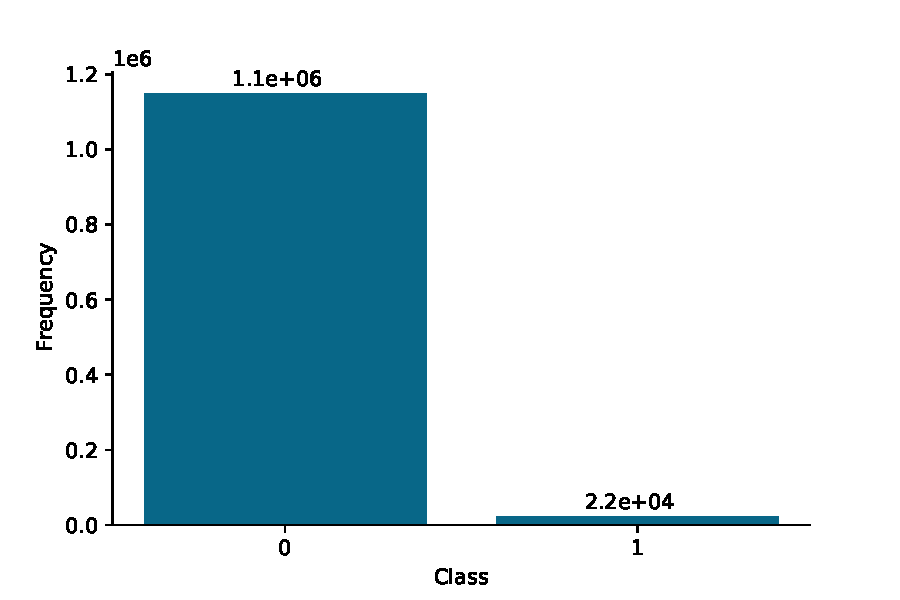
\includegraphics[scale = 0.7]{Label_dist.pdf}
    \caption{Breakdown of Target Variable}
    \label{fig:label_dist}
\end{figure}

\par The data that is used in the model consists of vital signs, laboratory values and demographic variables. We share some summarized statistics in Table \ref{tab_describe}. The vital signs includes data such as heart rate, pulse oximetry, temperature and systolic blood pressure. These vital signs are collected on a more regular basis and hence we can clearly see that they have less missing values. The laboratory values are the result from blood and other tests. Here we have variables such as fraction of inspired oxygen and glucose. A patient is not always tested and hence we can clearly see that this data is way sparser than those for the vital signs. The behavior of the missing is even clearer when looking at Figure \ref{fig:var_missings}. Figure \ref{fig:var_dists} gives us the distributions of the continuous variables. Here we see that most variables are normal or log normally distributed. 

\begin{table}
\centering
\caption{Summary Statistics}
\label{tab_describe}
\begin{tabular}{lcccccc}
\toprule
{} &   Mean & Standard Deviation &  Minimum & Median & Maximum & Percent Missing \\
\midrule
Heart Rate (bpm)                 &  84.75 &              17.20 &    20.00 &  84.00 &  280.00 &            0.09 \\
Pulse oximetry (\%)               &  97.21 &               2.93 &    20.00 &  98.00 &  100.00 &            0.13 \\
Temperature (Celsius)            &  36.99 &               0.78 &    20.90 &  37.00 &   42.22 &            0.66 \\
Systolic blood pressure (mm Hg)  & 122.75 &              22.69 &    20.00 & 120.00 &  296.00 &            0.15 \\
Mean arterial pressure (mm Hg)   &  81.13 &              15.97 &    20.00 &  79.00 &  300.00 &            0.12 \\
Diastolic blood pressure (mm Hg) &  62.78 &              13.68 &    20.00 &  61.00 &  300.00 &            0.37 \\
Respiration Rate (bpm)           &  18.75 &               5.22 &     1.00 &  18.00 &  100.00 &            0.14 \\
Fraction of inspired oxygen (\%)  &   0.56 &              11.50 &     0.00 &   0.50 & 4000.00 &            0.90 \\
Serum glucose (mg/dL)            & 136.24 &              51.56 &    10.00 & 126.00 &  988.00 &            0.85 \\
ICU length-of-stay               &  27.07 &              28.69 &     1.00 &  21.00 &  336.00 &            0.00 \\
Type of ICU                      &   0.50 &               0.50 &     0.00 &   1.00 &    1.00 &            0.43 \\
Age                              &  62.34 &              16.29 &    14.00 &  64.24 &  100.00 &            0.00 \\
Gender                           &   0.57 &               0.50 &     0.00 &   1.00 &    1.00 &            0.00 \\
Hospital Admission Time          & -54.65 &             167.17 & -5366.86 &  -4.92 &   23.99 &            0.00 \\
\bottomrule
\end{tabular}
\end{table}


\begin{figure}[htbp!]
    \centering
    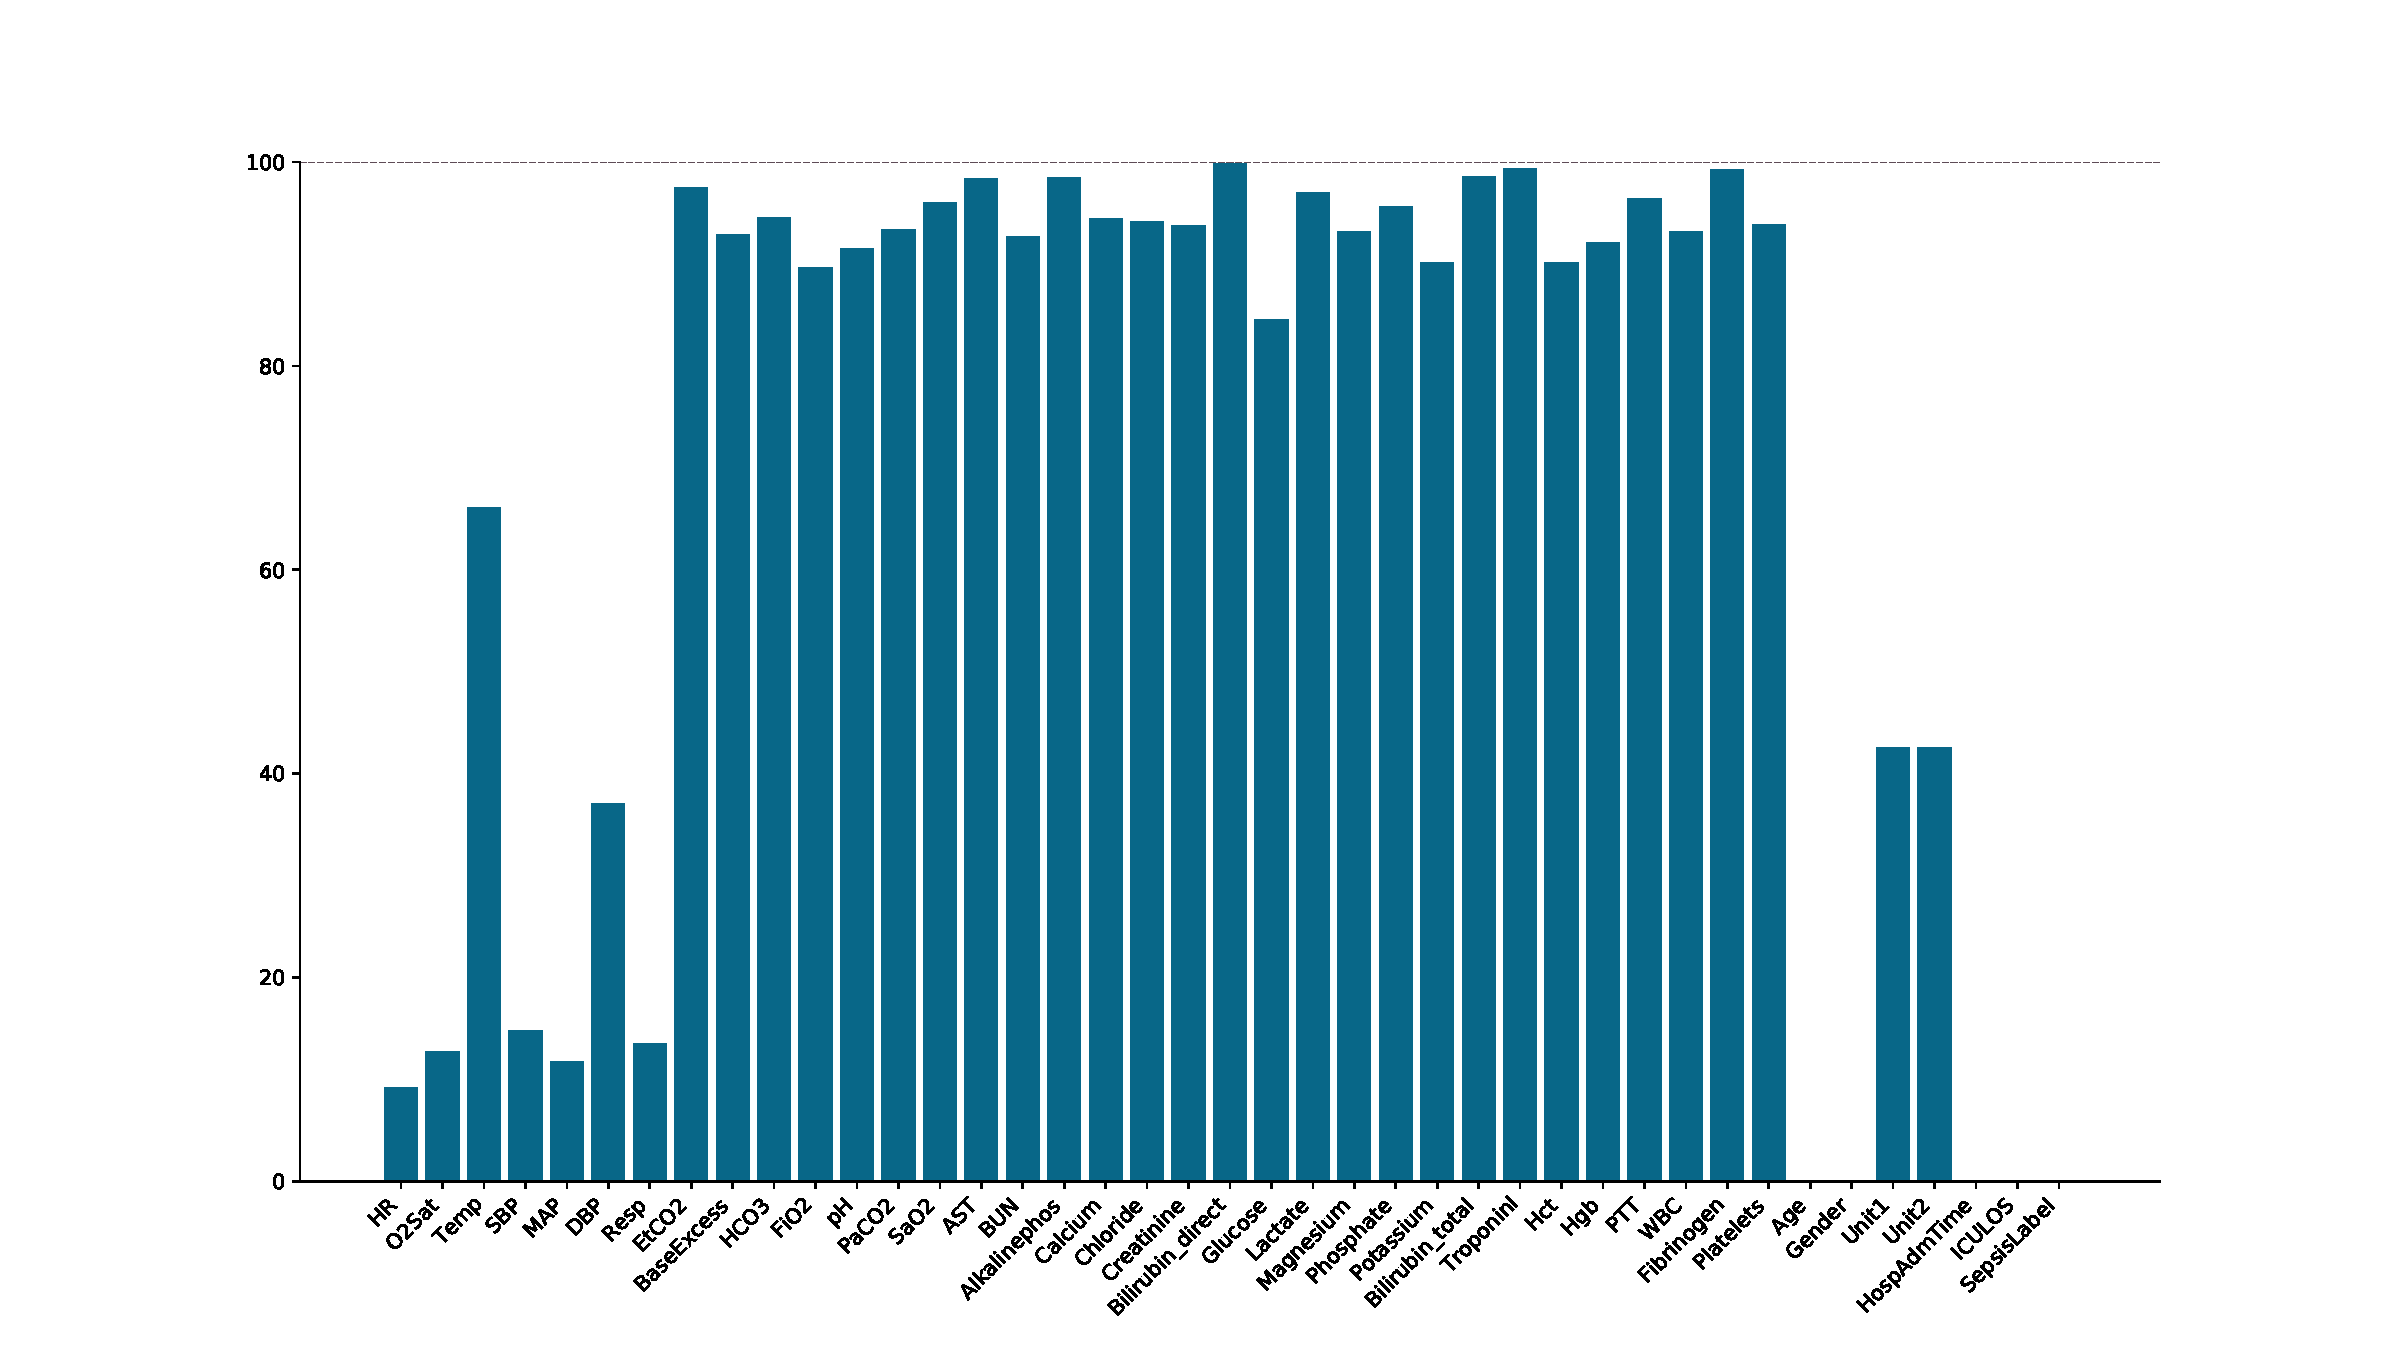
\includegraphics[scale = 0.45]{var_missing_hist.pdf}
    \caption{Percentage Missing per Variable}
    \label{fig:var_missings}
\end{figure}

\begin{figure}[htbp!]
    \centering
    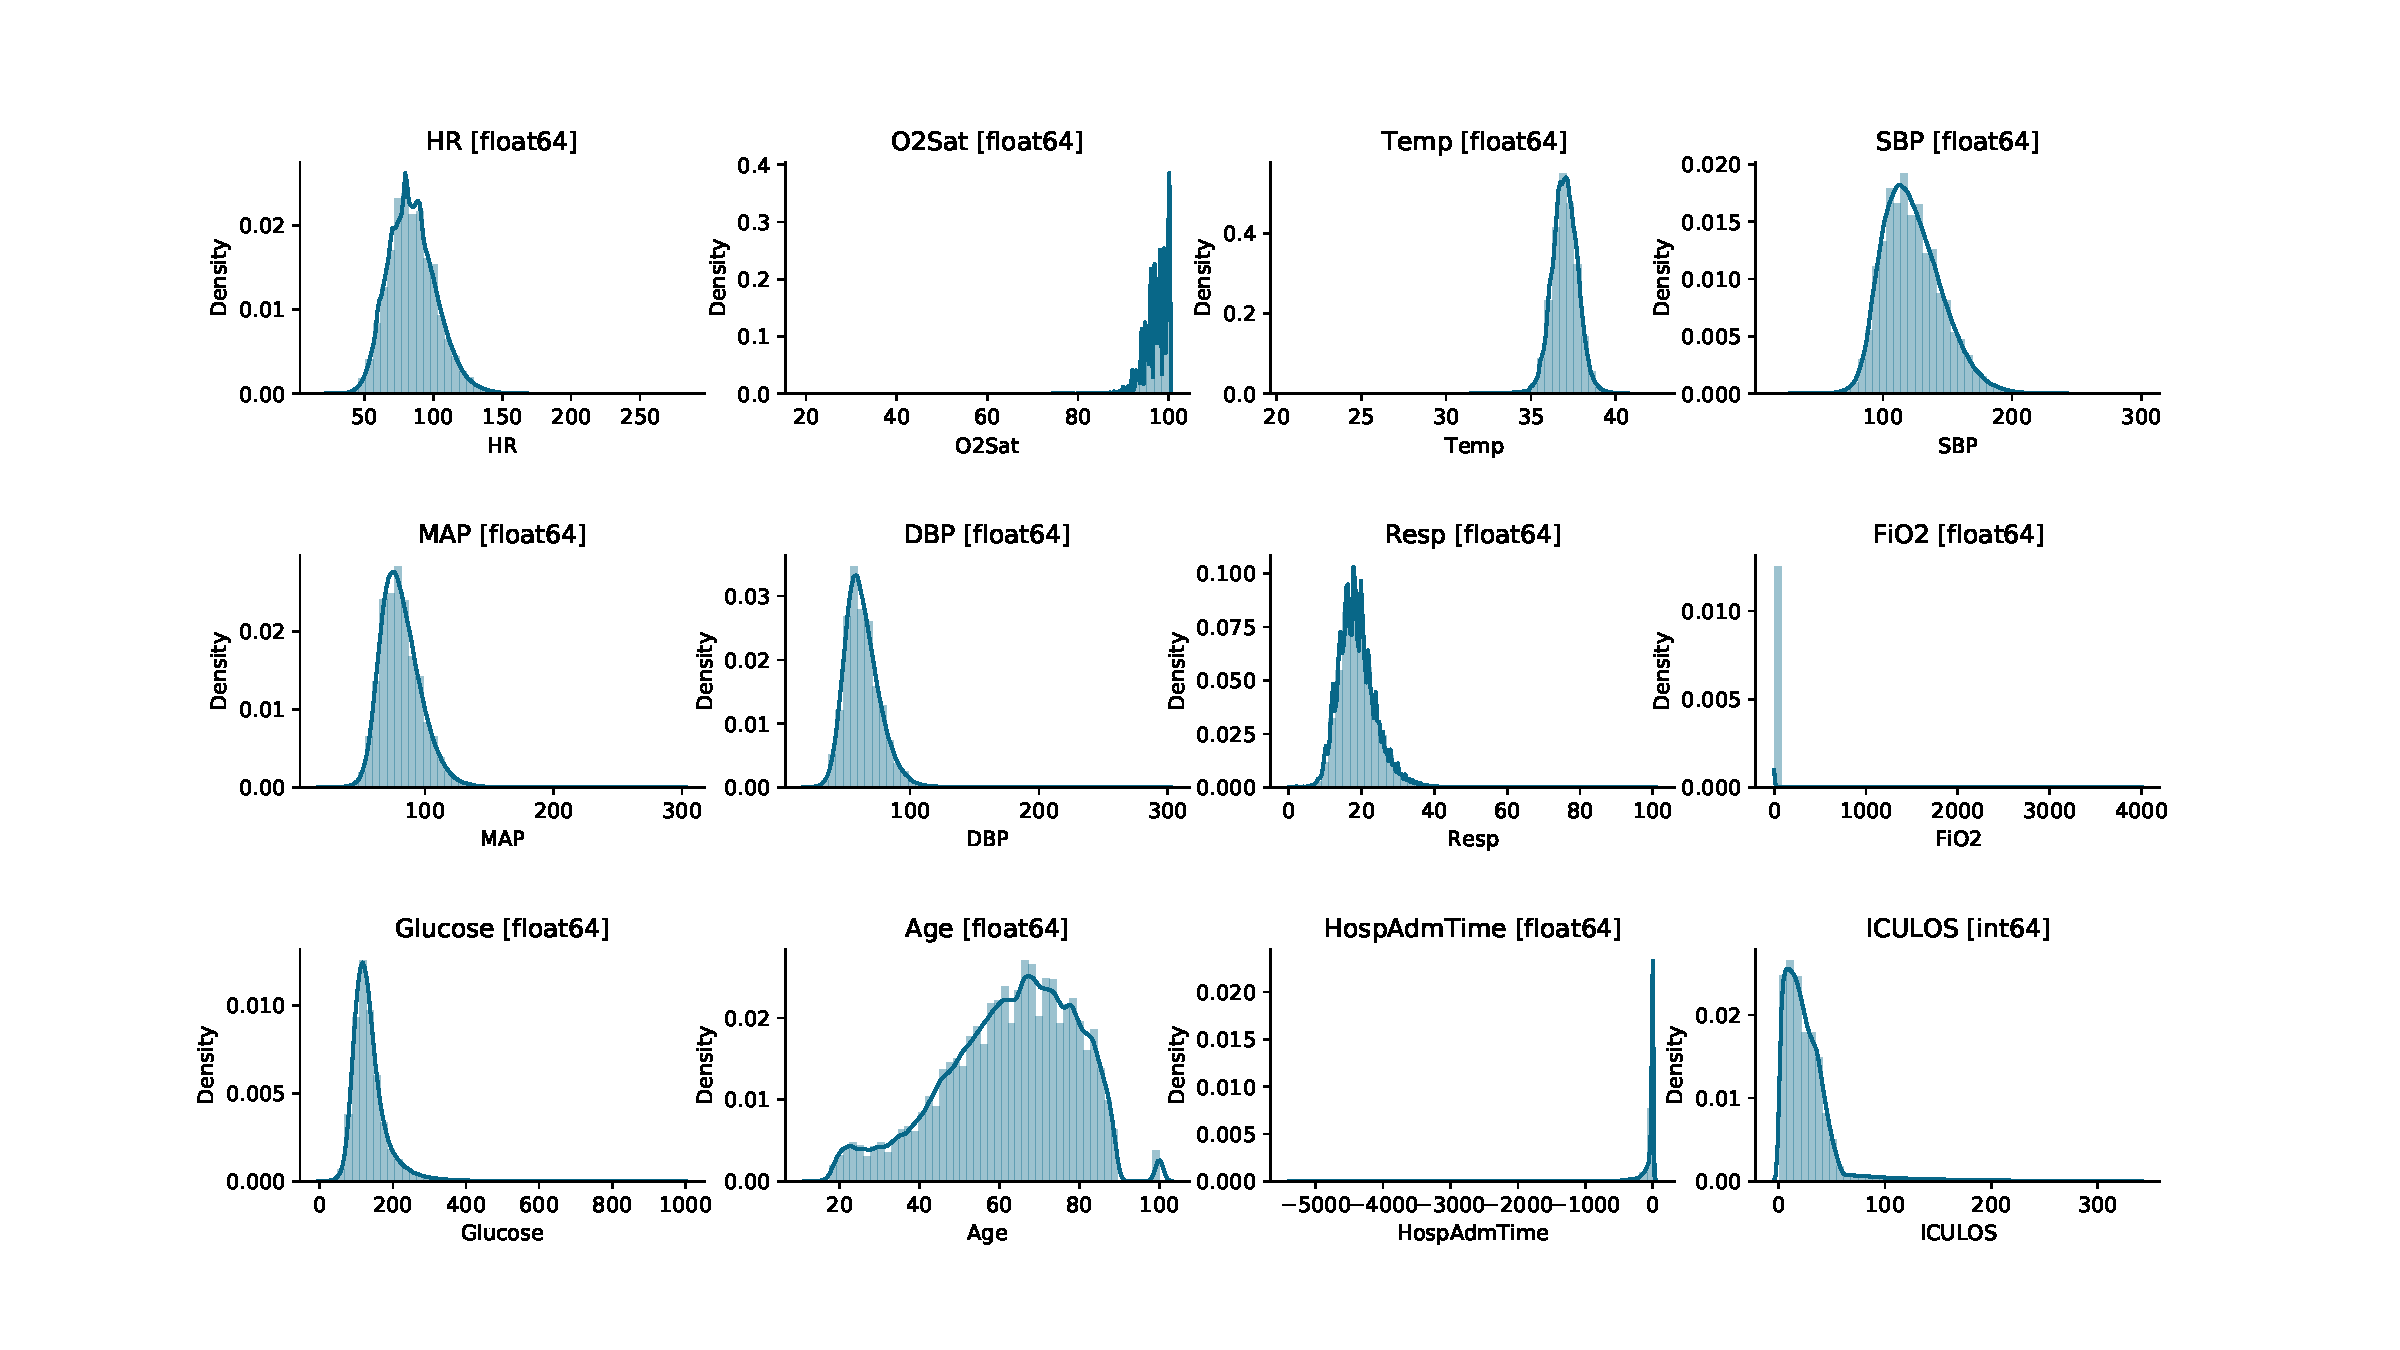
\includegraphics[scale = 0.45]{var_dists.pdf}
    \caption{Distributions of Continuous Variables}
    \label{fig:var_dists}
\end{figure}

\par An important aspect we need to look at is the breakdowns of the sepsis label per category. Our data has two categories we take into account. One is the gender which we will consider when evaluating fairness and the other is the type of ICU (either surgical or medical). We can see the breakdown of the labels in figures \ref{fig:label_ICU} and \ref{fig:label_per_sex}. We can see that you are 75\% and 12\% more likely to have sepsis in the medical ICU or as a male respectively. Another point that is valuable to make here, is that we can see that for every woman in the data set there are 1.3 men. This means that men are over-represented in the sample.

\begin{figure}[hbtp!]
\centering
\begin{subfigure}[b]{0.45\textwidth}
    \centering
    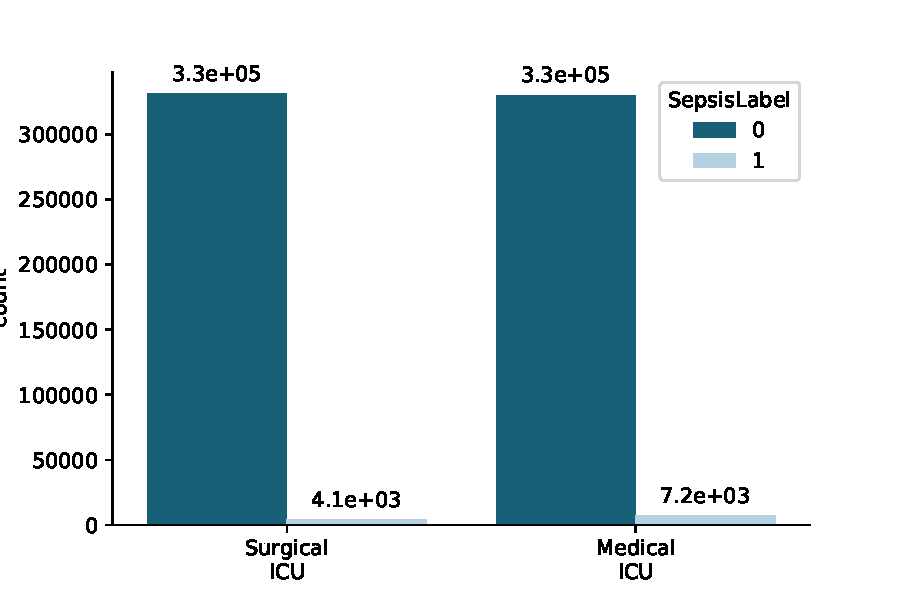
\includegraphics[scale = 0.6]{label_ICU.pdf}
    \caption{Type of ICU}
    \label{fig:label_ICU}
\end{subfigure}
\begin{subfigure}[b]{0.45\textwidth}
    \centering
    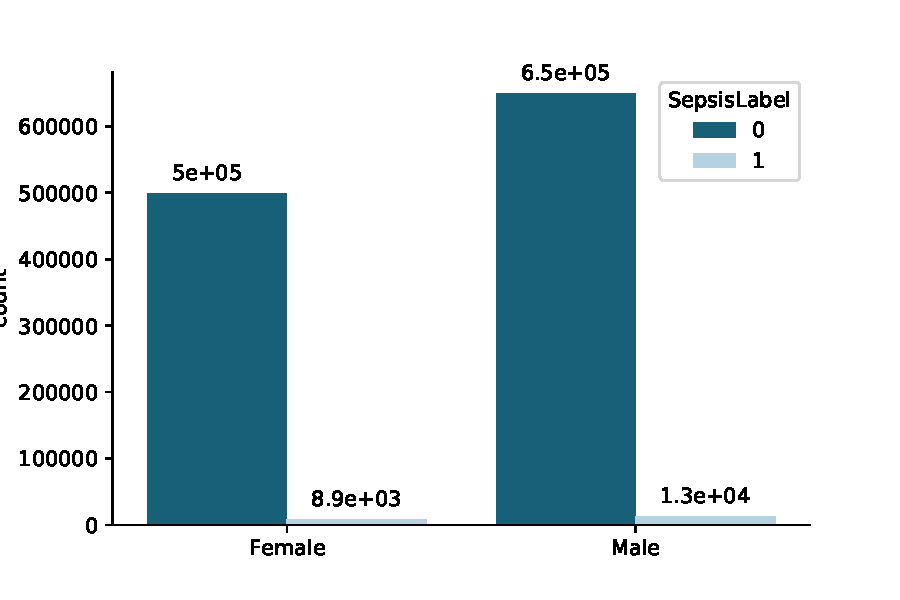
\includegraphics[scale = 0.6]{label_per_sex.pdf}
    \caption{Gender}
    \label{fig:label_per_sex}
\end{subfigure}
\caption{Sepsis by Categorical Variables}
\end{figure}

\par When looking at the correlation heatmap shown in Figure \ref{fig:corr_plot} we can see some interesting patterns. One is the very high correlation between the three types of blood pressure we are including and the strictly negative correlation between Unit1 and Unit2 which represent the medical and surgical ICU respectively. Something interesting to notice here is that there is a high correlation between temperature and being in the medical ICU and a high correlation between blood pressure and being in the surgical ICU. Another intuitively acceptable negative correlation is between the saturation of oxygen in the blood (O2Sat) and the respiratory rhythm (Resp). The more people need to breath the less oxygen would be available in their current blood. We also notice that an older patient in general seems to have a lower blood pressure than a young patient. 

\begin{figure}[htpb!]
    \centering
    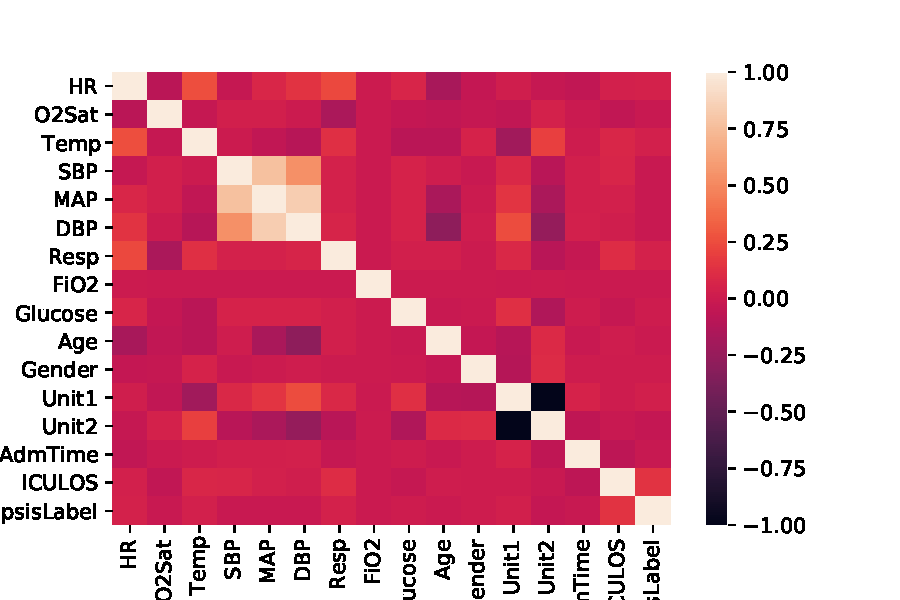
\includegraphics[scale = 0.7]{corr_plot.pdf}
    \caption{Correlation Plot}
    \label{fig:corr_plot}
\end{figure}

\section*{Implementation and validation}

% DEVELOP A DETAILED PLAN FOR THE OTHER SECTIONS:

% 3. Implementation and validation: present your understanding of the code that implements the ADS. This code was implemented by others (e.g., as part of the Kaggle competition), not by you as part of this assignment. Your goal here is to demonstrate that you understand the implementation at a high level.
%	a. Describe data cleaning and any other pre-processing
%	b. Give high-level information about the implementation of the system
%	c. How was the ADS validated? How do we know that it meets its stated goal(s)?

\section*{Outcomes}

% 4. Outcomes
%	a. Analyze the effectiveness (accuracy) of the ADS by comparing its performance across different subpopulations.
%	b. Select one or several fairness or diversity measures, justify your choice of these measures for the ADS in question, and quantify the fairness or diversity of this ADS.
%	c. Develop additional methods for analyzing ADS performance: think about stability, robustness, performance on difficult or otherwise important examples (in the style of LIME), or any other property that you believe is important to check for this ADS.

\section*{Summary}

% 5. Summary
%	a. Do you believe that the data was appropriate for this ADS?
%	b. Do you believe the implementation is robust, accurate, and fair? Discuss your choice of accuracy and fairness measures, and explain which stakeholders may find these measures appropriate.
%	c. Would you be comfortable deploying this ADS in the public sector, or in the industry? Why so or why not?
%	d. What improvements do you recommend to the data collection, processing, or analysis methodology?




\newpage
\bibliographystyle{apacite}
\bibliography{references}
\end{document}